\documentclass[preview,border=12pt]{standalone}
\usepackage{parskip}
\usepackage{tikz}
\usepackage{pifont}
\usepackage{graphicx}
\usepackage[utf8]{inputenc}
\usepackage[T1]{fontenc}
\usepackage[swedish]{babel}
\begin{document}
\setlength{\parskip}{0pt}
\pgfmathsetmacro{\cardroundingradius}{4mm}
\pgfmathsetmacro{\striproundingradius}{3mm}
\pgfmathsetmacro{\cardwidth}{5}
\pgfmathsetmacro{\cardheight}{8}
\newcommand{\stripcolor}{cyan}
\pgfmathsetmacro{\stripwidth}{1.2}
\pgfmathsetmacro{\strippadding}{0.1}
\newcommand{\striptext}{FEM FYRFOTA \rotatebox[origin=c]{-90}{\ding{49}}}
\pgfmathsetmacro{\textpadding}{0.3}
\newcommand{\topcaption}{SNUTTAN}
%\newcommand{\topcontent}{\textit{''Jamande kattväsen'}}
%\newcommand{\bottomcaption}{Kompisar}
\newcommand{\bottomcontent}{
			\begin{list}{}{\leftmargin=0em \itemindent=0em}
				\item Alfred
				\item Bina
				\item Hönsen
				\item Udda
			\end{list}
			\vspace{1.0cm}
			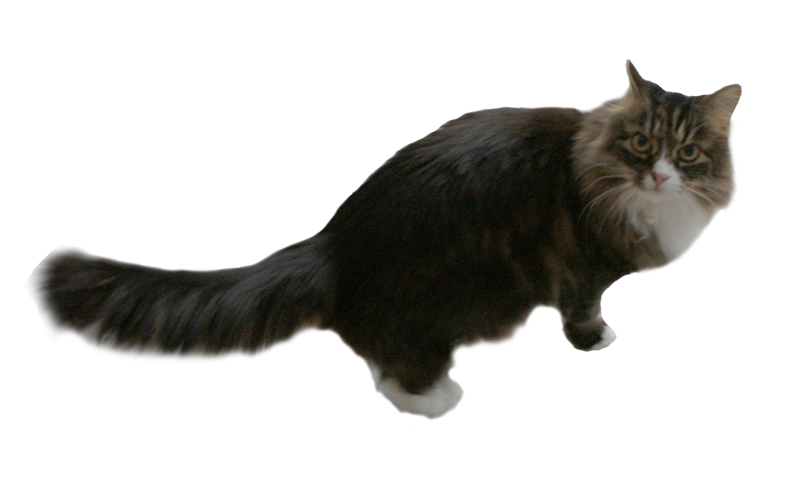
\includegraphics[width=\textwidth]{snuttan.png}
}
\pgfmathsetmacro{\ruleheight}{0.1}
\newcommand{\stripfontsize}{\Huge}
\newcommand{\captionfontsize}{\LARGE}
\newcommand{\textfontsize}{\large}
\begin{tikzpicture}
    \draw[rounded corners=\cardroundingradius] (0,0) rectangle (\cardwidth,\cardheight);
    \fill[\stripcolor,rounded corners=\striproundingradius] (\strippadding,\strippadding) rectangle (\strippadding+\stripwidth,\cardheight-\strippadding) node[rotate=90,above left,black,font=\stripfontsize] {\striptext};
    \node[text width=(\cardwidth-\strippadding-\stripwidth-2*\textpadding)*1cm,below right,inner sep=0] at (\strippadding+\stripwidth+\textpadding,\cardheight-\textpadding) 
    {   {\captionfontsize \topcaption}\\ 
        %{\textfontsize \topcontent}\\
		\tikz{\fill (0,0) rectangle (\cardwidth-\strippadding-\stripwidth-2*\textpadding,\ruleheight);}\\[0.3em]
        %{\captionfontsize \bottomcaption}\\ 
        {\textfontsize \bottomcontent}
    };
\end{tikzpicture}
\end{document}
